\documentclass[UTF8, a4paper, 11pt]{article}
\usepackage{diagbox}
\usepackage{subfigure}
\usepackage[UTF8, scheme=plain]{ctex}
\usepackage{fontspec}
\usepackage{float}
\usepackage{amsmath}
\newtheorem{myDef}{Definition}
\usepackage{graphicx}
\usepackage{geometry}
\usepackage{listings}
\usepackage{xcolor}
\usepackage{caption}
\geometry{scale=0.8}
\linespread{1.5}
\usepackage{hyperref}
\usepackage{color}
\usepackage{fontspec}
\usepackage{enumitem}
\usepackage[linesnumbered,boxed]{algorithm2e}    
\usepackage{xeCJK}
\usepackage{indentfirst} 
\graphicspath{{Pics/}} 	% 在于.tex同级的目录下创建名为pic的文件夹,存放图片


\setlength{\parindent}{2em}

\lstset{
    language={C},
    frame=shadowbox,
    breaklines=true,
    numbers=left,
    backgroundcolor=\color[RGB]{245,245,244},
    rulesepcolor=\color{red!20!green!20!blue!20},
    numberstyle={\color[RGB]{0,192,192}\tiny},
    basicstyle=\footnotesize \fontspec{Source Code Pro}
}
\setenumerate[1]{itemsep=0pt,partopsep=0pt,parsep=\parskip,topsep=0pt}
\setitemize[1]{itemsep=0pt,partopsep=0pt,parsep=\parskip,topsep=0pt}
\setdescription{itemsep=0pt,partopsep=0pt,parsep=\parskip,topsep=0pt}


\title{	
\normalfont \normalsize
\textsc{School of Data and Computer Science, Sun Yat-sen University} \\ [25pt] %textsc small capital letters
\rule{\textwidth}{0.5pt} \\[0.4cm] % Thin top horizontal rule
\huge 数电实验3\\ % The assignment title
\rule{\textwidth}{2pt} \\[0.5cm] % Thick bottom horizontal rule
\author{18308045 谷正阳}
\date{\normalsize\today}
}

\begin{document}
\maketitle
\tableofcontents
\newpage
\section{仿真实验}
\subsection{五位二进制码转格雷码}
\subsubsection{电路设计}
$$
G_i=
\begin{cases}
    Q_i\oplus Q_{i+1},&i=0,1,2,3\\
    Q_i,&i=4
\end{cases}
$$
在此5个输入分别用CLK1,Q0,Q1,Q2,Q3代替,输出结果应如下:
\begin{table}[H]
    \center
\begin{tabular}{|l|l|}
\hline
Q     & G     \\ \hline
00000 & 00000 \\ \hline
00001 & 00001 \\ \hline
00010 & 00011 \\ \hline
00011 & 00010 \\ \hline
00100 & 00110 \\ \hline
00101 & 00111 \\ \hline
00110 & 00101 \\ \hline
00111 & 00100 \\ \hline
01000 & 01100 \\ \hline
01001 & 01101 \\ \hline
01010 & 01111 \\ \hline
01011 & 01110 \\ \hline
01100 & 01010 \\ \hline
01101 & 01011 \\ \hline
01110 & 01001 \\ \hline
01111 & 01000 \\ \hline
10000 & 11000 \\ \hline
10001 & 11001 \\ \hline
10010 & 11011 \\ \hline
10011 & 11010 \\ \hline
10100 & 11110 \\ \hline
10101 & 11111 \\ \hline
10110 & 11101 \\ \hline
10111 & 11100 \\ \hline
11000 & 10100 \\ \hline
11001 & 10101 \\ \hline
11010 & 10111 \\ \hline
11011 & 10110 \\ \hline
11100 & 10010 \\ \hline
11101 & 10011 \\ \hline
11110 & 10001 \\ \hline
11111 & 10000 \\ \hline
\end{tabular}
\end{table}
\subsubsection{电路图}
\begin{figure}[H]
    \centering
    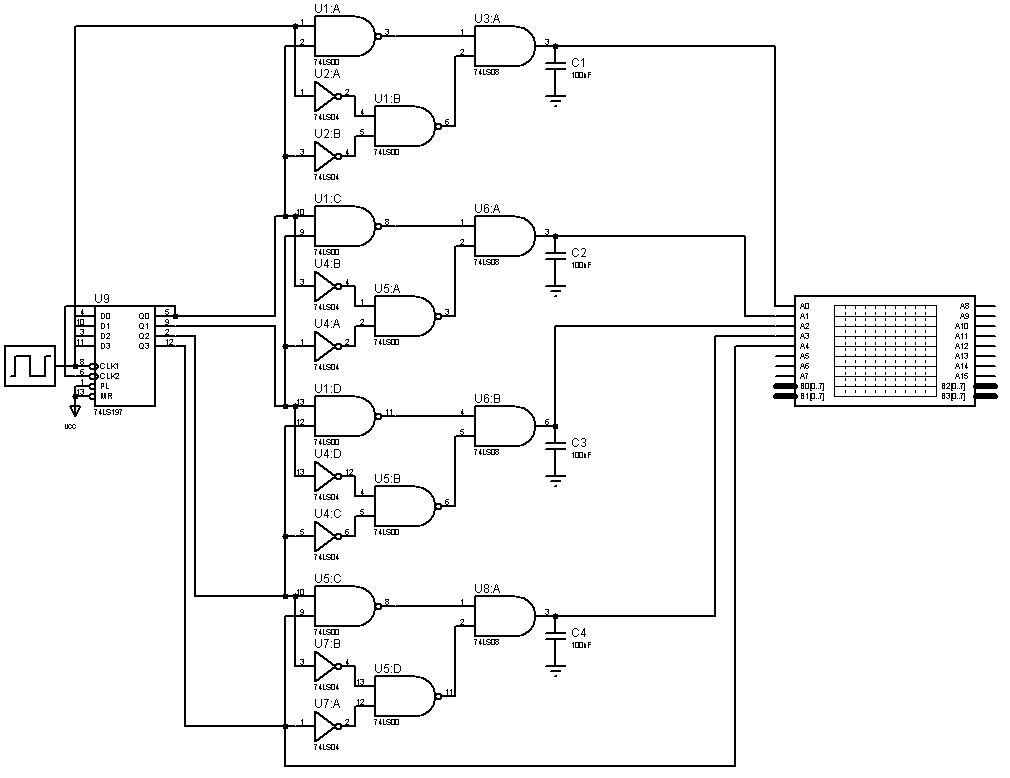
\includegraphics[width=0.8\textwidth]{ex3.1.jpg}
\end{figure}
电路中还使用了电容去除毛刺,因为异或门输入端AB同时变化时会出现竞争冒险现象。
\subsubsection{波形图}
\begin{figure}[H]
    \centering
    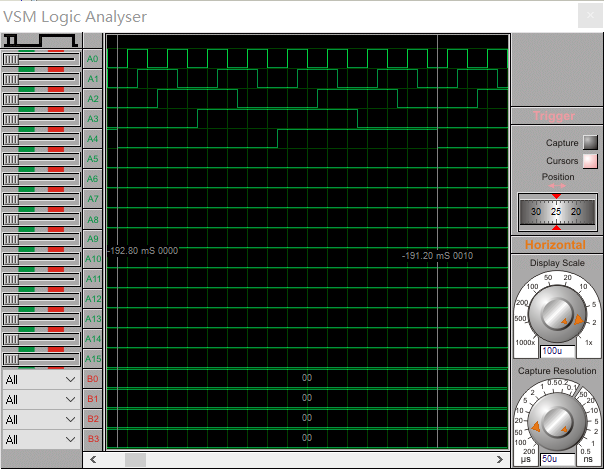
\includegraphics[width=0.8\textwidth]{ex3.1.png}
\end{figure}
符合预期。
\subsection{五位格雷码转二进制码}
\subsubsection{电路设计}
$$
Q_i=
\begin{cases}
    G_i\oplus Q_{i+1},&i=0,1,2,3\\
    G_i,&i=4
\end{cases}
$$
在此5个输入分别用CLK1,Q0,Q1,Q2,Q3代替,输出结果应如下:
\begin{table}[H]
    \center
\begin{tabular}{|l|l|}
\hline
G      & Q      \\ \hline
000000 & 000000 \\ \hline
000001 & 000001 \\ \hline
000010 & 000011 \\ \hline
000011 & 000010 \\ \hline
000100 & 000111 \\ \hline
000101 & 000110 \\ \hline
000110 & 000100 \\ \hline
000111 & 000101 \\ \hline
001000 & 001111 \\ \hline
001001 & 001110 \\ \hline
001010 & 001100 \\ \hline
001011 & 001101 \\ \hline
001100 & 001000 \\ \hline
001101 & 001001 \\ \hline
001110 & 001011 \\ \hline
001111 & 001010 \\ \hline
010000 & 011111 \\ \hline
010001 & 011110 \\ \hline
010010 & 011100 \\ \hline
010011 & 011101 \\ \hline
010100 & 011000 \\ \hline
010101 & 011001 \\ \hline
010110 & 011011 \\ \hline
010111 & 011010 \\ \hline
011000 & 010000 \\ \hline
011001 & 010001 \\ \hline
011010 & 010011 \\ \hline
011011 & 010010 \\ \hline
011100 & 010111 \\ \hline
011101 & 010110 \\ \hline
011110 & 010100 \\ \hline
011111 & 010101 \\ \hline
\end{tabular}
\end{table}
\subsubsection{电路图}
\begin{figure}[H]
    \centering
    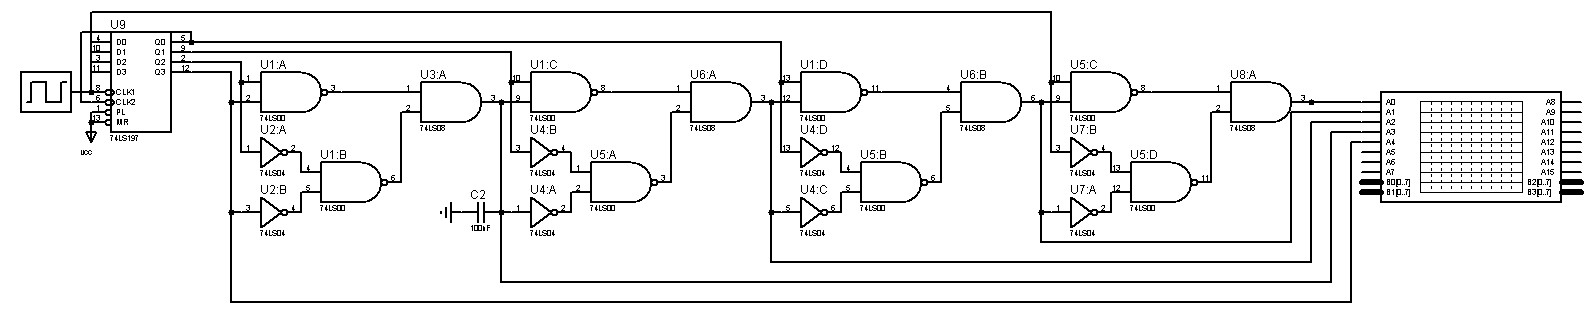
\includegraphics[width=0.8\textwidth]{ex3.2.jpg}
\end{figure}
在此未使用电容处理毛刺,因为层数太多无法处理。
\subsubsection{波形图}
\begin{figure}[H]
    \centering
    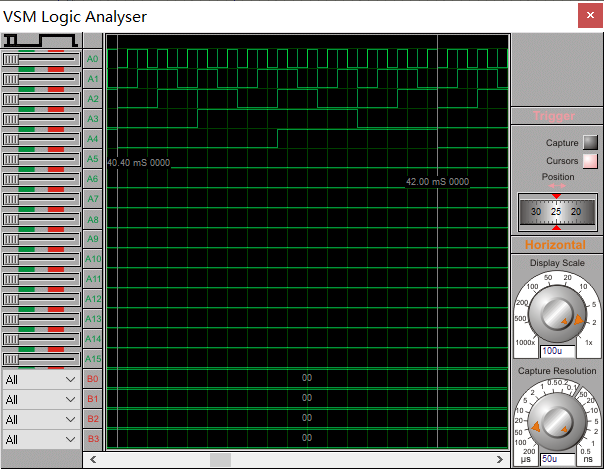
\includegraphics[width=0.8\textwidth]{ex3.2.png}
\end{figure}
\subsection{四位二进制码转7段码}
\subsubsection{电路设计}
在此运用了三八译码器的思想,使用16个4输入的与门和一些非门实现了高电平有效的四十六译码器。再将其与共阴极的七段数码管相连。
\subsubsection{电路图}
\begin{figure}[H]
    \centering
    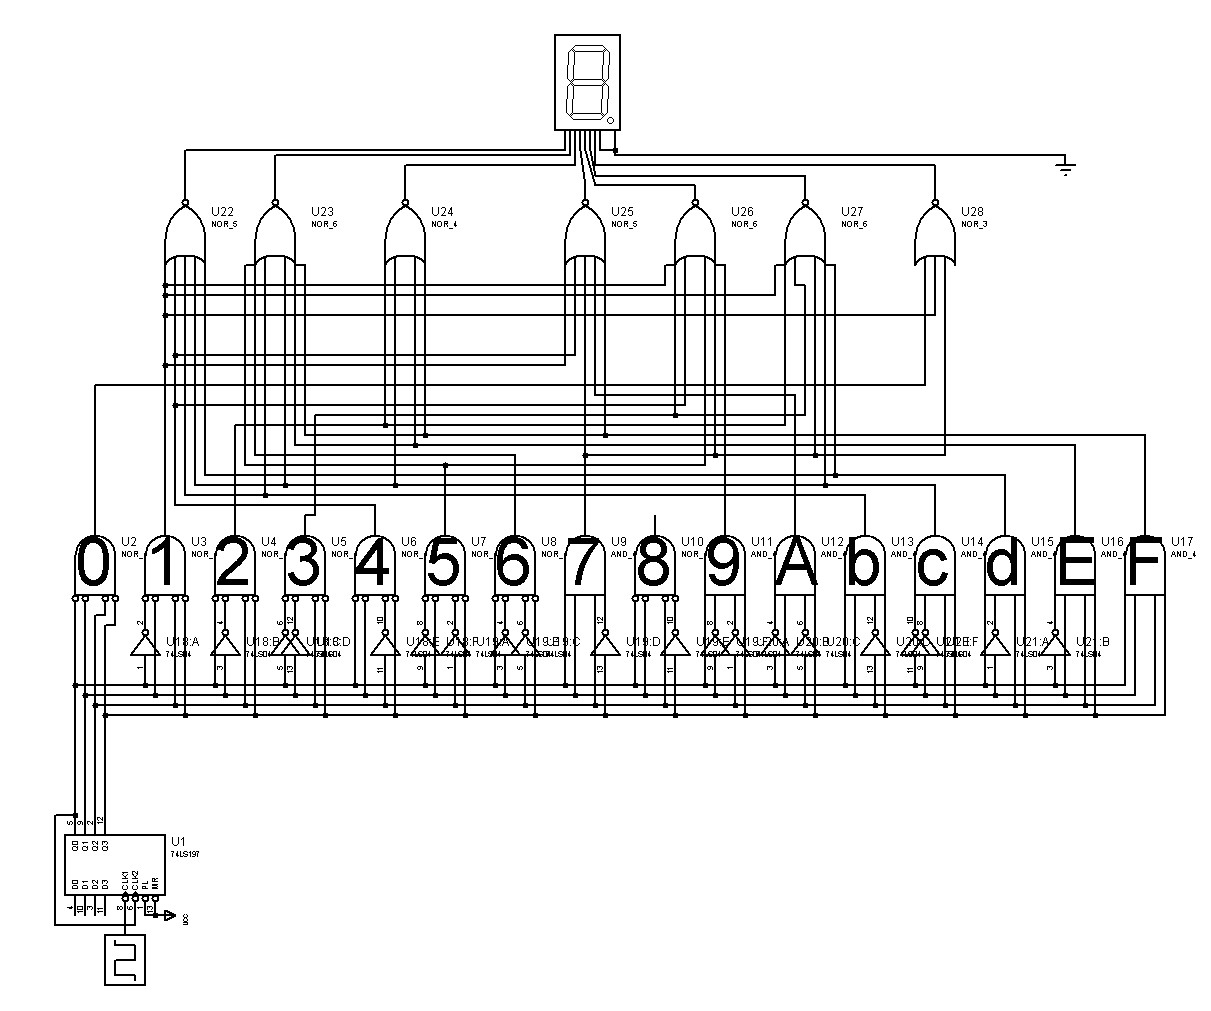
\includegraphics[width=0.8\textwidth]{ex3.3.jpg}
\end{figure}
在此未使用电容处理毛刺,因为层数太多无法处理。
\subsubsection{演示视频}
\href{run:/Vids/ex3.3.mp4}{ex3.3.mp4}
\section{实验箱实验}
\subsection{五位二进制码转格雷码}
\begin{figure}[H]
    \centering
    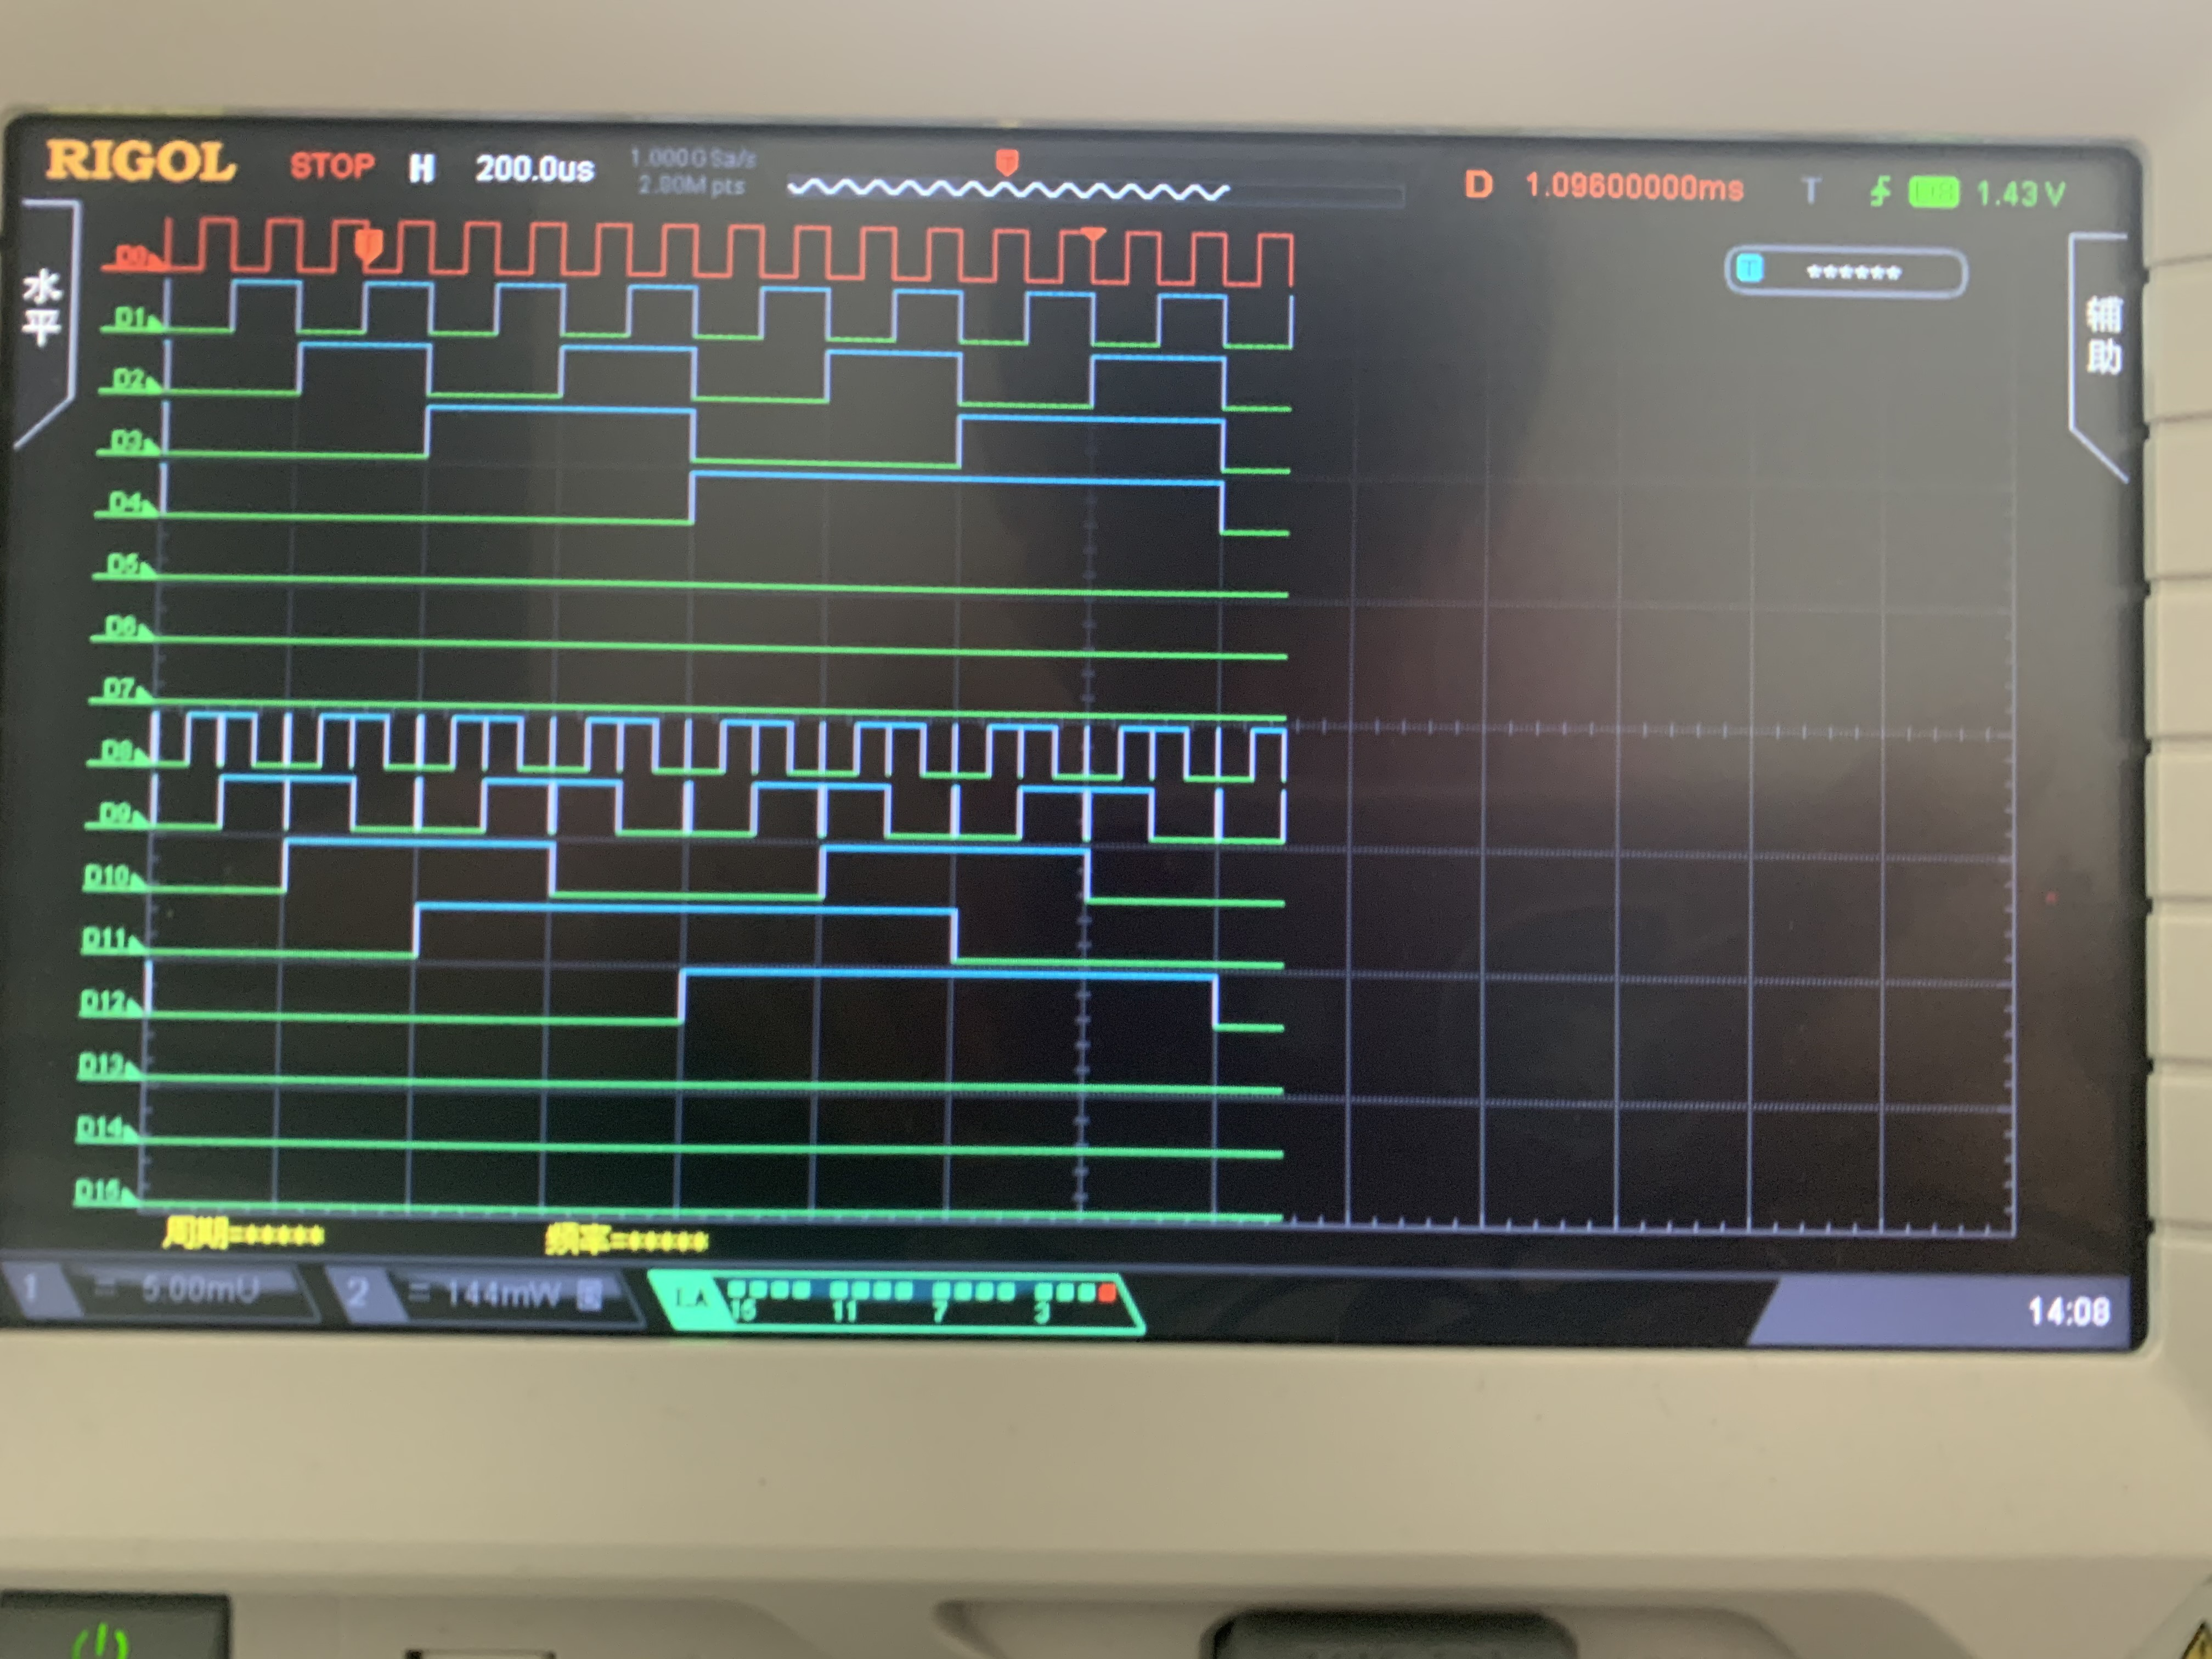
\includegraphics[width=0.8\textwidth]{Q2G.JPG}
\end{figure}
\subsection{五位格雷码转二进制码}
\begin{figure}[H]
    \centering
    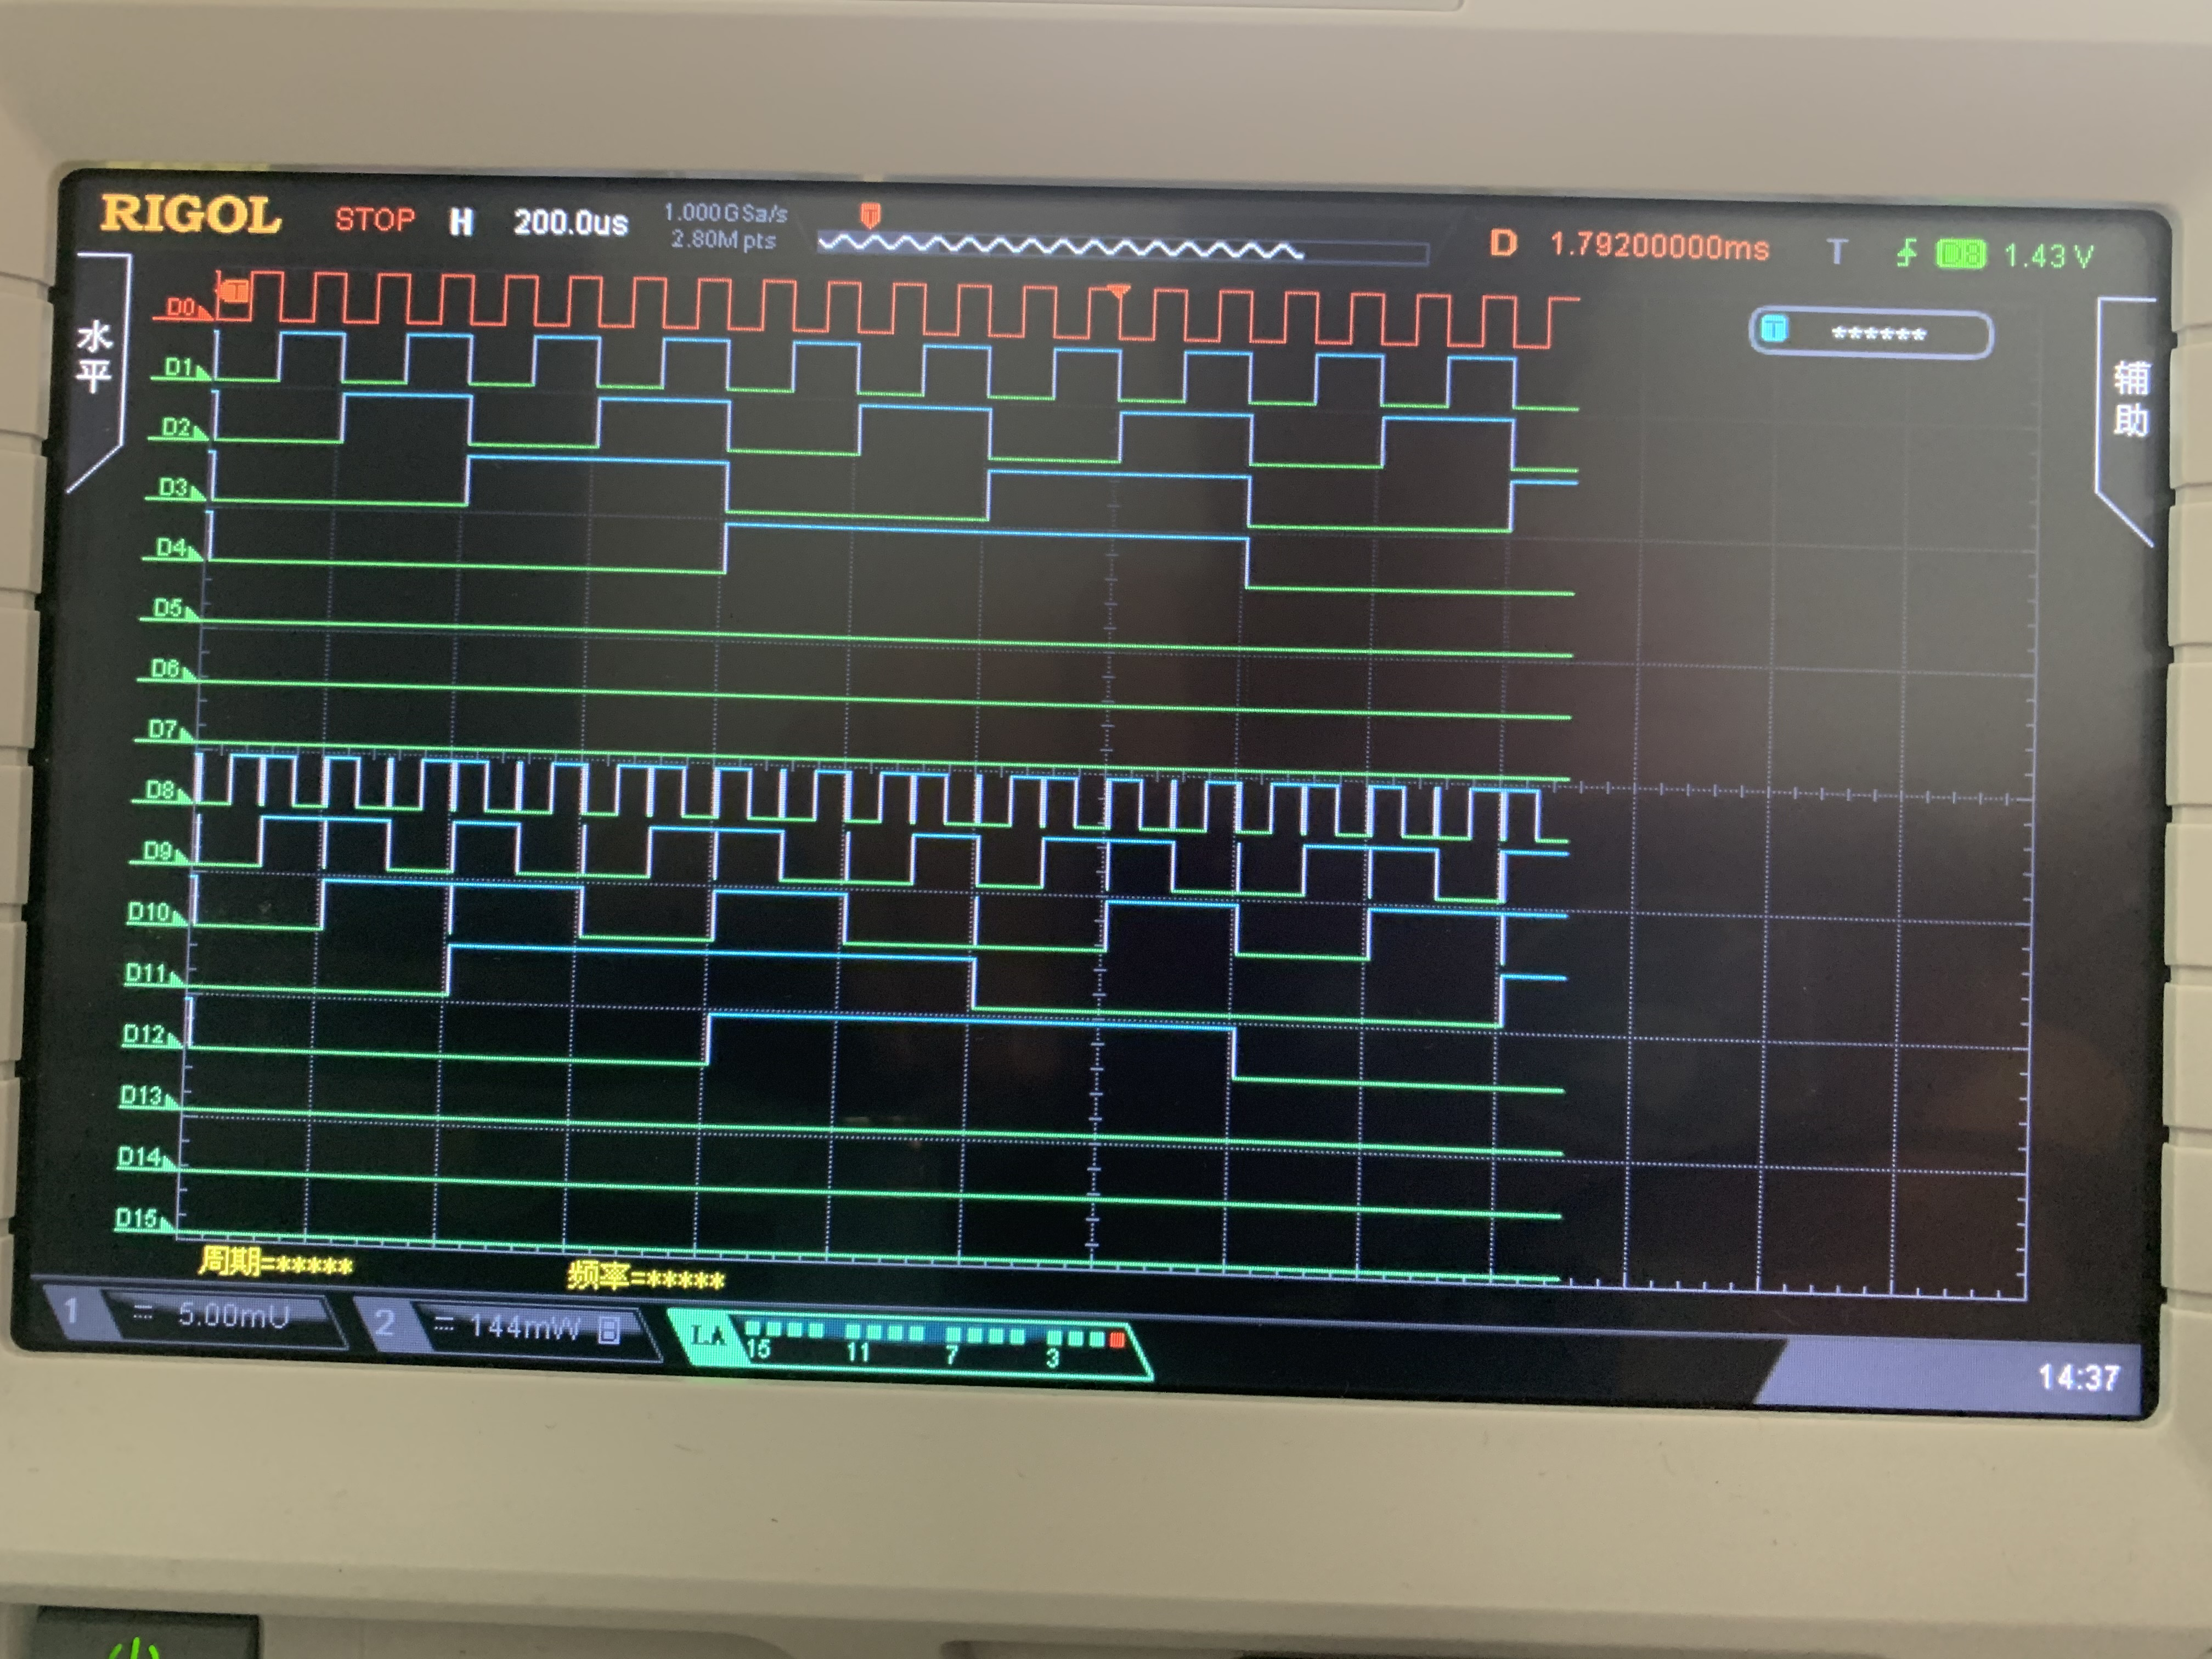
\includegraphics[width=0.8\textwidth]{G2Q.JPG}
\end{figure}
\section{实验总结}
学会设计一些电路。
%\clearpage
%\bibliography{E:/Papers/LiuLab}
%\bibliographystyle{apalike}
\end{document}
%%% Local Variables:
%%% mode: latex
%%% TeX-master: t
%%% End:
